\section{Benchmark problem 1: offshore strip footing loading}\label{sec:example1}\noindent
\subsection{FE model setup}\noindent
To evaluate the proposed metamodel, a strip footing loading problem on silty sand was considered, featuring low-dimensional static inputs and high-dimensional, multi-stage, multi-field outputs. Numerical simulations were performed using the commercial software ABAQUS \parencite{abaqus2022}. The model geometry and mesh configuration are shown in \Cref{fig: Mesh}, where the strip footing is represented by an equivalent surface loading \parencite{houlsby1999,xiao2018,haghighi2019}. The footing width is $D = 1.9$ m, and the soil-footing interface is assumed rough without separation, consistent with the undrained condition \parencite{yang2021,huang2021,yang2022,zhou2023,yang2024,peng2025,wang2025} . The soil layer is idealised as homogeneous, governed by a Mohr Coulomb failure criterion under total stress analysis. Loading is applied via prescribed loading, divided into nine increments of 7 kPa each, representing multi-stage loading. To minimise boundary effects, domain extents are set as $B_V=3D$ vertically and $B_H=4.5D$ horizontally. A mesh convergence study indicated that a minimum element size of $0.05D$ was sufficient for accuracy. Plane strain conditions were assumed, and the soil domain was discretised using 4-node bilinear quadrilateral elements. Boundary conditions were applied by fixing the bottom and lateral edges, while symmetry was enforced along the model centre-line using roller constraints. A geostatic equilibrium step was first performed to establish the initial in-situ stress field under gravity. The displacement field was subsequently reset to zero prior to applying the strip footing load, ensuring that the computed response corresponds solely to the applied loading.
\setcounter{figure}{5} 

To construct the metamodel, two geotechnical parameters were considered as input variables: the elastic modulus stiffness ratio, $E/s_u \sim \mathcal{U}(40,\ 2000)$, and the undrained shear strength, $s_u \sim \mathcal{U}(8\ \mathrm{kPa},\ 50\ \mathrm{kPa})$. The remaining non-linear parameters were kept constant, with the friction angle and dilation angle fixed at 28$^\circ$ and 2$^\circ$, respectively. Two output regions were extracted from the numerical results at each loading stage: (i) the ground surface zone adjacent to the footing and (ii) the subsoil zone directly beneath the footing. The former yields a vector-based output comprising 21 nodes along the surface, while the latter provides a field-based output defined over a $21 \times 17$ grid in the vertical cross-section. Each simulation consists of 9 loading increments, resulting in two output tensors:
$\tilde{\mathcal{M}}: x \in \mathbb{R}^{1 \times 2}  \rightarrow 
\mathcal{G}^{(1)} \in \mathbb{R}^{9*21}$ for surface vectors, and
$\tilde{\mathcal{M}}: x \in \mathbb{R}^{1 \times 2}  \rightarrow 
\mathcal{G}^{(2)} \in \mathbb{R}^{9*21*17} $ for subsoil fields,
where $\mathbb{R}^{1 \times 2}$ represents the input space defined by $E/s_u$ and $s_u$. $\mathcal{G}$ denotes the type of different fields of output quantities. This benchmark problem is designed to demonstrate the metamodel’s ability to capture spatially and temporally evolving geotechnical responses. 

While the current model setup considers only two input parameters ($E/s_u$ and $s_u$) and assumes a homogeneous soil layer, this simplification serves as a proof-of-concept to validate the proposed method on a simplified offshore strip footing scenario. The framework can easily extend and readily accommodate additional geotechnical input parameters, more complex constitutive models, non-linear relationships, as well as spatial variability and stratified or heterogeneous ground conditions in future applications.
\begin{figure}
\centering
 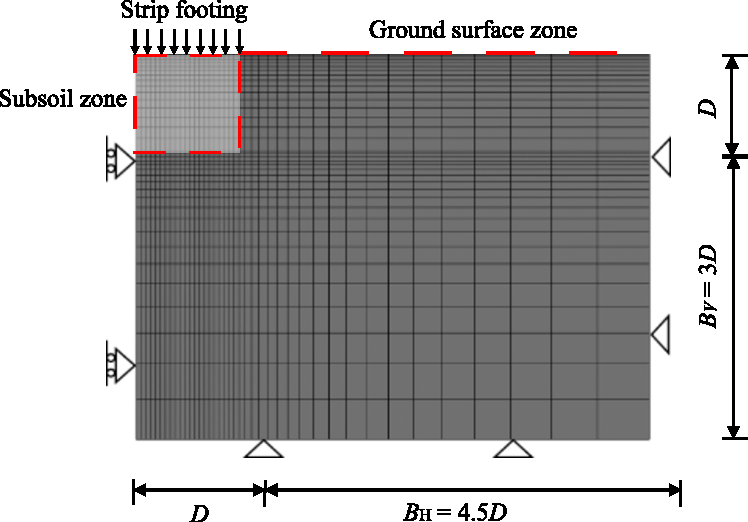
\includegraphics[width=90mm]{main_images/figure-stripfooting.pdf}
 \caption{FE model}
 \label{fig: Mesh}
\end{figure}



\subsection{Metamodel details}\noindent
The metamodel architecture is shown in \Cref{tab:nn_architecture1}. It begins with a fully connected layer comprising 50 hidden units, which maps the static input parameters into a latent feature space. The resulting latent representation is repeated across the nine loading stages and fed into an LSTM module to capture temporal dependencies. The LSTM output is then decoded into two separate branches corresponding to the two output types. Latin Hypercube sampling was used to generate 350 samples from the defined parameter space $\mathcal{D}_{\boldsymbol{x}}$. For all simulations, the dataset is partitioned using a fixed random seed. For the learning-curve analysis, subsets corresponding to 16\%, 24\%, 32\%, 40\% and 80\% of the full dataset are used for training, while the remaining 20\% samples form a fixed test set and are not used during training. The input parameters and model responses are then normalised to $[0,1]$ globally using a min-max transformation, with the scaling factors estimated from the training pool and applied unchanged to the test set. For each response quantity, the spatio-temporal tensors are flattened to arrays of size $(n_{\text{sample}}, N_{\text{dof}})$ prior to scaling and subsequently reshaped to their original dimensions.



The first branch reconstructs the ground surface settlement $\mathcal{G}^{(1)}$ using a sequence of time-distributed transposed 1D convolution layers. The latent sequence is first passed through a dense layer of 320 units and reshaped into a temporal sequence, followed by convolution layers with kernel size 3, stride 2, and ReLU activation. The second branch reconstructs the subsoil displacement field $\mathcal{G}^{(2)}$ using time-distributed transposed 2D convolution layers. The latent vector is first expanded through a dense layer into a spatial tensor, then reshaped and processed by convolution layers with 64, 32, 16, and 1 filters, all with kernel size 3, stride 1, and 'same' padding. ReLU activation is used for all layers except the final one, which uses linear activation to preserve continuous field values. Both branches are trained jointly using a unified loss function and Adam optimiser on \texttt{Tensorflow} API, allowing consistent learning across vector and field outputs. The hyperparameters, such as the number of hidden units, were empirically chosen based on the complexity of the task and the dimensionality of the output sequences. This choice balances predictive accuracy and hyper-parameter tuning complexities. Although further optimisation could improve performance, this configuration suffices to demonstrate the method's feasibility. It is noted that no explicit physics constraints, such as those in Physics-Informed Neural Networks, were used; however, the outputs were checked for physical plausibility. Convergence challenges, which may arise in geotechnical problems with large displacements or non-linear behaviour, could be addressed by adjusting step sizes and refining the mesh in critical regions.
\begin{table}[t]
\centering
\caption{Neural network architecture and parameter counts for offshore strip footing problem}
\label{tab:nn_architecture1}
\small
\setlength{\tabcolsep}{5pt}
\begin{tabular}{lll r}
\toprule
Layer & Type & Output shape & Params \\
\midrule
Input & InputLayer & (None, 2) & 0 \\
Dense & Dense(50) & (None, 50) & 150 \\
Repeat & RepeatVector(9) & (None, 9, 50) & 0 \\
LSTM & LSTM(50), return\_seq & (None, 9, 50) & 20{,}200 \\
\midrule
\multicolumn{4}{c}{\textbf{Branch A: displacement vector output}} \\
\midrule
TD-Dense & TimeDistributed(Dense(320)) & (None, 9, 320) & 16{,}320 \\
TD-Reshape & TimeDistributed(Reshape) & (None, 9, 10, 32) & 0 \\
TD-Conv1DT & TimeDistributed(Conv1DTranspose(1)) & (None, 9, 21, 1) & 97 \\
Output-A & Lambda (squeeze) & (None, 9, 21) & 0 \\
\midrule
\multicolumn{4}{c}{\textbf{Branch B: displacement field output}} \\
\midrule
TD-Dense & TimeDistributed(Dense(1344)) & (None, 9, 1344) & 68{,}544 \\
TD-Reshape & TimeDistributed(Reshape) & (None, 9, 16, 21, 4) & 0 \\
TD-Conv2DT-1 & TimeDistributed(Conv2DTranspose(64)) & (None, 9, 16, 21, 64) & 2{,}368 \\
TD-Conv2DT-2 & TimeDistributed(Conv2DTranspose(32)) & (None, 9, 16, 21, 32) & 18{,}464 \\
TD-Conv2DT-3 & TimeDistributed(Conv2DTranspose(16)) & (None, 9, 16, 21, 16) & 4{,}624 \\
TD-Conv2DT-4 & TimeDistributed(Conv2DTranspose(1)) & (None, 9, 16, 21, 1) & 145 \\
Output-B & Lambda (squeeze) & (None, 9, 16, 21) & 0 \\
\midrule
\textbf{Total} &  &  & \textbf{130{,}912} \\
\bottomrule
\end{tabular}
\end{table}

\subsection{Baselines}\noindent
To evaluate the predictive capability of the proposed surrogate model, comparisons are conducted against several established baseline approaches in order to place its performance in context. All models are trained and assessed using the same dataset partitioning and evaluation metrics to ensure consistency. As a representative reduced-order modelling (ROM) strategy, a PCA-PCE framework is adopted. In this approach, principal component analysis (PCA) is employed as a matrix-based dimensionality reduction technique to extract dominant modes from the high-dimensional output field; the spatial outputs are therefore flattened prior to decomposition and reshaped back to their original configuration after reconstruction. Polynomial chaos expansion (PCE) is subsequently used to establish the mapping between input parameters and the reduced coefficients, following the implementation described in \cite{yang2026}. In addition to this baseline, component-wise model configurations of the proposed architecture are constructed to examine the contributions of individual components. Specifically, the LSTM layers are removed to assess the role of temporal feature extraction in capturing time-dependent behaviour, while a separate variant without convolution layers is developed to evaluate the influence of CNN-based spatial feature learning on representing complex spatial patterns and local interactions within the predicted field. These controlled comparisons enable the respective contributions of reduced-order modelling, temporal learning, and spatial feature extraction to be examined in a consistent framework.


\subsection{Metamodel performance}\noindent
The predictive performance of the metamodel is quantified by comparison with reference simulations using the \textit{Global Normalised Absolute Error} (GNAE, a normalised $L_1$ type error), \textit{Mean Absolute Error} (MAE) and \textit{Relative $L_2$ Error} ($L_2$ type error) \parencite{chai2014,mendo2009,zhu2019}, defined as follows:
\begin{equation}
 \text{GNAE} = \frac{1}{K'} \sum_{k=1}^{K'} \frac{ \left| \mathcal{M}(x_k) - \tilde{\mathcal{M}}(x_k) \right| } {\max(\mathcal{M}(x_k)) - \min(\mathcal{M}(x_k))} \times 100 , 
\end{equation}
\begin{equation}
\text{MAE}
=
\frac{1}{K'}
\sum_{k=1}^{K'}
\left|
\mathcal{M}(x_k) - \tilde{\mathcal{M}}(x_k)
\right|, 
\end{equation}
\begin{equation}
\text{Relative } L_2
=
\frac{
\sqrt{
\sum_{k=1}^{K'}
\left(
\mathcal{M}(x_k)
-
\tilde{\mathcal{M}}(x_k)
\right)^2
}
}
{
\sqrt{
\sum_{k=1}^{K'}
\left(
\mathcal{M}(x_k)
\right)^2
}
}
, 
\end{equation}
where $K'$ denotes the number of FE simulations in the test set, $\mathcal{M}(x)$ represents the FE predictions, and $\tilde{\mathcal{M}}(x)$ denotes the corresponding metamodel outputs. The GNAE provides a scale-independent percentage measure by normalising the absolute error with respect to the global range of the reference solution. This normalisation enhances robustness when the solution magnitude varies significantly across the domain and reduces the influence of disproportionately large local deviations. The MAE quantifies the average magnitude of pointwise prediction errors, offering a direct and physically interpretable assessment of absolute deviation. It reflects the typical local discrepancy between the predicted and reference values without overemphasising extreme errors. The Relative $L_2$ error evaluates the global error in an energy-norm sense by considering the squared differences between prediction and reference.

The evolution of the loss over training epochs is illustrated in \Cref{fig: loss}, where a logarithmic scale is employed to emphasise the rapid reduction in the early stages of training. As expected, the total loss decreases progressively, spanning approximately three orders of magnitude over the entire training period. The loss associated with $\mathcal{G}^{(1)}$ stabilises relatively quickly, likely due to the lower spatial complexity and smoother nature of its output, which is a vector. In contrast, the loss corresponding to $\mathcal{G}^{(2)}$ exhibits evident fluctuations and a slower convergence rate, attributable to the higher spatial complexity of the predicted field. From a physical standpoint, this behaviour is consistent with the role of $\mathcal{G}^{(2)}$ in capturing complex and spatially detailed variations within the subsoil displacement field. Despite these challenges, the overall trend, along with the eventual plateauing of the loss, indicates that the model has reached convergence.

The test performance of the different surrogate models under varying training sample sizes is summarised in \Cref{tab:test_error1,tab:test_error2,tab:test_error3}. For both the vector-valued response $\mathcal{G}^{(1)}$ and the field-type response $\mathcal{G}^{(2)}$, a general reduction in all three error measures (GNAE, MAE and $L_2$) is observed as the number of training samples increases, indicating that all models benefit from additional high-fidelity data. In which, the PCA-PCE model performs reasonably well at smaller sample sizes but its accuracy improves only modestly as further data are added, suggesting that its capacity to capture the strong non-linearity and spatio-temporal coupling in the present problem is limited. The comparison among the three neural-network baselines further clarifies the role of the different components in the proposed architecture: the CNN+MLP configuration without LSTM systematically underperforms the recurrent variants, highlighting that neglecting temporal dynamics leads to an inferior representation of sequence-dependent responses, whereas the “LSTM Only” configuration improves the treatment of temporal correlations but, owing to the absence of an explicit convolution layer, lacks the ability to efficiently exploit spatial structure and therefore yields an intermediate level of accuracy between CNN+MLP and the full proposed model. Overall, these observations indicate that the proposed architecture is necessary to exploit both spatial and temporal dependencies effectively. Three complementary error measures, GNAE, MAE and the $L_2$, are employed to mitigate the risk of drawing misleading conclusions from a single metric; although their absolute magnitudes differ, they provide consistent rankings of the competing surrogates over all sample sizes and for both output types, thereby offering a robust assessment of the superiority and reliability of the proposed model. \Cref{fig: fitting} shows regression plots comparing the metamodel predictions of $\mathcal{G}^{(1)}$ and $\mathcal{G}^{(2)}$ with the corresponding reference values for both training and test datasets, with the diagonal line indicating perfect agreement. In all cases, the points lie in a narrow band around the identity line, and no systematic bias, trend reversal or noticeable outliers can be observed between training and test sets, suggesting that over-fitting is negligible.  

\begin{figure}
\centering
 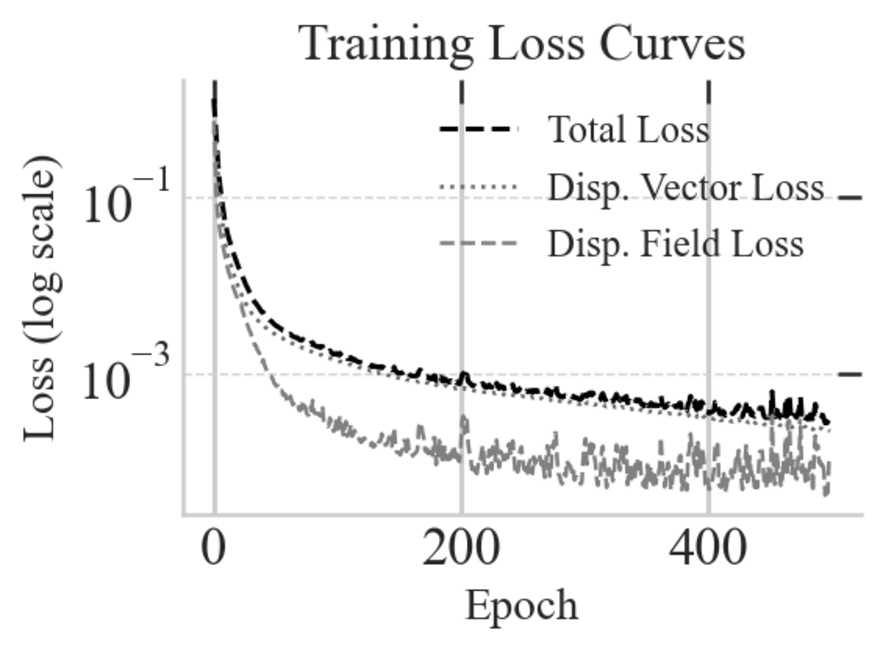
\includegraphics[width=90mm]{main_images/figure-loss.pdf}
 \caption{Training loss curves for total and output-specific losses}
 \label{fig: loss}
\end{figure}




\begin{table}[htbp]
\centering
\caption{GNAE of different surrogate models under varying training sample sizes}
\label{tab:test_error1}
\sisetup{
    table-format=3.2,
    detect-weight=true,
    detect-inline-weight=math
}
\begin{tabular}{c l S S S S}
\toprule
\multirow{2}{*}{Samples} & \multirow{2}{*}{Case} & 
\multicolumn{4}{c}{Test Error (\%)} \\
\cmidrule(lr){3-6}
 &  & {Proposed} & {PCA--PCE} & {CNN+MLP (No LSTM)} & {LSTM Only} \\
\midrule
56  & $\mathcal{G}^{(1)}$ & 4.05 & 4.21 & 9.80 & 5.02 \\
84  & $\mathcal{G}^{(1)}$ & 2.30 & 3.38 & 10.78 & 4.24 \\
112 & $\mathcal{G}^{(1)}$ & 2.01 & 3.10 & 10.70 & 2.51 \\
140 & $\mathcal{G}^{(1)}$ & 1.56 & 3.00 & 9.86 & 2.87 \\
280 & $\mathcal{G}^{(1)}$ & 1.27 & 3.24 & 7.36 & 3.03 \\
\midrule
56  & $\mathcal{G}^{(2)}$ & 5.50 & 7.16 & 8.57 & 5.65 \\
84  & $\mathcal{G}^{(2)}$ & 6.17 & 4.57 & 7.32 & 3.74 \\
112 & $\mathcal{G}^{(2)}$ & 4.53 & 4.26 & 6.54 & 3.27 \\
140 & $\mathcal{G}^{(2)}$ & 6.55 & 4.15 & 6.14 & 2.81 \\
280 & $\mathcal{G}^{(2)}$ & 0.82 & 4.35 & 6.12 & 2.93 \\
\bottomrule
\end{tabular}
\end{table}


\begin{table}[htbp]
\centering
\caption{MAE of different surrogate models under varying training sample sizes}
\label{tab:test_error2}
\sisetup{
    table-number-alignment = center,
    table-format = 1.2
}
\begin{tabular}{c c S S S S}
\toprule
\multirow{2}{*}{Samples} & \multirow{2}{*}{Case} &
\multicolumn{4}{c}{Test Error} \\
\cmidrule(lr){3-6}
 & & {Proposed} & {PCA--PCE} & {CNN+MLP (No LSTM)} & {LSTM Only} \\
\midrule
56  & $\mathcal{G}^{(1)}$ & 0.07 & 0.07 & 0.17 & 0.09 \\
84  & $\mathcal{G}^{(1)}$ & 0.04 & 0.06 & 0.19 & 0.07 \\
112 & $\mathcal{G}^{(1)}$ & 0.03 & 0.05 & 0.18 & 0.04 \\
140 & $\mathcal{G}^{(1)}$ & 0.03 & 0.05 & 0.17 & 0.05 \\
280 & $\mathcal{G}^{(1)}$ & 0.02 & 0.05 & 0.13 & 0.04 \\
\midrule
56  & $\mathcal{G}^{(2)}$ & 0.39 & 0.51 & 0.61 & 0.40 \\
84  & $\mathcal{G}^{(2)}$ & 0.44 & 0.32 & 0.52 & 0.27 \\
112 & $\mathcal{G}^{(2)}$ & 0.32 & 0.30 & 0.46 & 0.23 \\
140 & $\mathcal{G}^{(2)}$ & 0.47 & 0.29 & 0.43 & 0.20 \\
280 & $\mathcal{G}^{(2)}$ & 0.06 & 0.30 & 0.23 & 0.18 \\
\bottomrule
\end{tabular}
\end{table}


\begin{table}[htbp]
\centering
\caption{$L_2$ of different surrogate models under varying training sample sizes}
\label{tab:test_error3}
\sisetup{
    table-number-alignment = center,
    table-format = 1.2
}
\begin{tabular}{c c S S S S}
\toprule
\multirow{2}{*}{Samples} & \multirow{2}{*}{Case} &
\multicolumn{4}{c}{Test Error} \\
\cmidrule(lr){3-6}
 & & {Proposed} & {PCA--PCE} & {CNN+MLP (No LSTM)} & {LSTM Only} \\
\midrule
56  & $\mathcal{G}^{(1)}$ & 0.09 & 0.05 & 0.12 & 0.10 \\
84  & $\mathcal{G}^{(1)}$ & 0.03 & 0.04 & 0.11 & 0.04 \\
112 & $\mathcal{G}^{(1)}$ & 0.03 & 0.03 & 0.10 & 0.03 \\
140 & $\mathcal{G}^{(1)}$ & 0.02 & 0.04 & 0.10 & 0.03 \\
280 & $\mathcal{G}^{(1)}$ & 0.01 & 0.04 & 0.08 & 0.03 \\
\midrule
56  & $\mathcal{G}^{(2)}$ & 0.10 & 0.07 & 0.11 & 0.11 \\
84  & $\mathcal{G}^{(2)}$ & 0.05 & 0.04 & 0.06 & 0.04 \\
112 & $\mathcal{G}^{(2)}$ & 0.04 & 0.04 & 0.06 & 0.03 \\
140 & $\mathcal{G}^{(2)}$ & 0.05 & 0.04 & 0.06 & 0.03 \\
280 & $\mathcal{G}^{(2)}$ & 0.01 & 0.04 & 0.07 & 0.03 \\
\bottomrule
\end{tabular}
\end{table}


As an illustration, \Cref{fig: output} shows representative responses of both the metamodel and the forward model in the original output space. For the vector-type output $\mathcal{G}^{(1)}$, \Cref{fig: output}(a) demonstrates that the predicted profiles (red lines) align well with the reference FE results (black lines) over all loading stages, correctly reproducing both the magnitude and the shape of the settlement. For the field-type output $\mathcal{G}^{(2)}$, \Cref{fig: output}(b) shows the numerical model displacement fields, the corresponding metamodel prediction and their point-wise differences at three representative stages (1, 5 and 9). As the load increases, the true fields exhibit a progressive expansion and deepening of the deformation zone beneath and around the footing, and the metamodel closely follows this evolution. The error maps show small, spatially scattered residuals with no evident systematic bias. Overall, the agreement between the metamodel and FE solutions is satisfactory in both space and time, and the remaining discrepancies are small relative to the response magnitude and acceptable for typical geotechnical applications.

\begin{figure}[htbp]
    \centering
    \begin{subfigure}[b]{\textwidth}
        \centering
        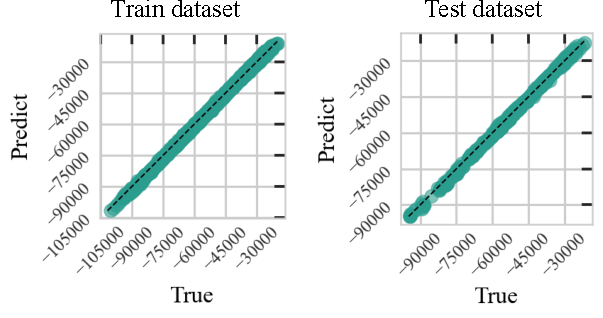
\includegraphics[width = 90mm]{main_images/figure-G1.pdf}
        \caption{$\mathcal{G}^{(1)}$}
    \end{subfigure}%
    \vfill
    \begin{subfigure}[b]{\textwidth}
        \centering
        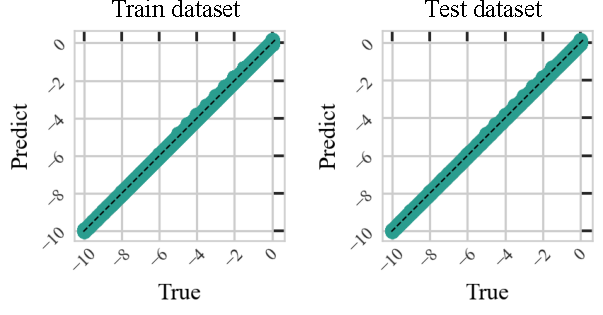
\includegraphics[width = 90mm]{main_images/figure-G2.pdf}
        \caption{$\mathcal{G}^{(2)}$}
    \end{subfigure}%
    \caption{Regression plot}
    \label{fig: fitting}
\end{figure}


To facilitate surrogate modelling and maintain reproducibility, the workflow was implemented in an end-to-end manner. Input parameters were sampled evenly using the Latin Hypercube sampling method, and for each parameter set, a FE simulation was performed to obtain the corresponding model responses. The outputs from all simulations were collected and reshaped into arrays suitable for neural network training, with vector-type responses arranged as rows and field-type outputs as matrix. The dataset was divided into training and validation subsets (80\% and 20\%, respectively) using a fixed random seed, and all inputs and outputs were scaled to the [0,1] range using min-max normalisation before training. The surrogate was trained on these preprocessed data, with a fixed seed ensuring consistent weight initialisation and mini-batch sampling. Once trained, the NN was used in a sequential calibration framework, where Markov Chain Monte Carlo sampling was performed to approximate the soil parameters' distributions; fixed seeds were applied here as well. By following this sequence, from design space sampling and FE simulation, through data reshaping, normalisation, and NN training, to surrogate-based calibration, the procedure can be reproduced under comparable computational conditions.

\begin{figure}[htbp]
    \centering
    \begin{subfigure}[b]{\textwidth}
        \centering
        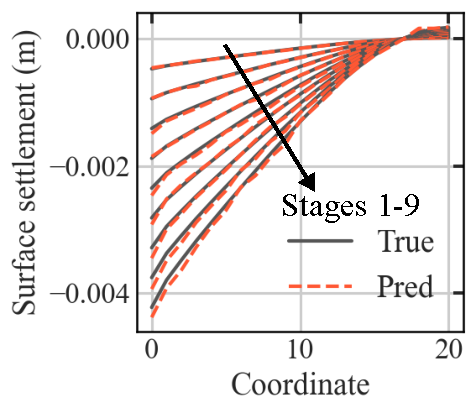
\includegraphics[width = 70mm]{main_images/figure-G1output.pdf}
        \caption{$\mathcal{G}^{(1)}$}
    \end{subfigure}%
    \vfill
    \begin{subfigure}[b]{\textwidth}
        \centering
        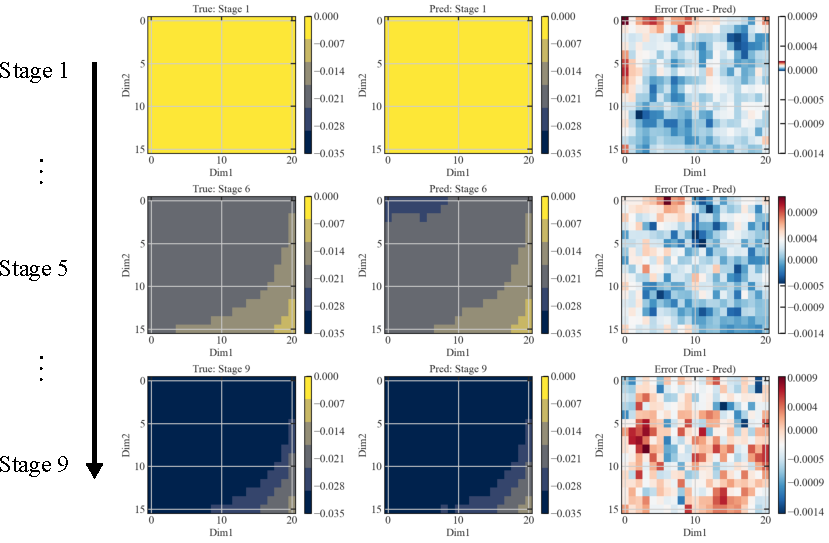
\includegraphics[width = 140mm]{main_images/figure-G2output.pdf}
        \caption{$\mathcal{G}^{(2)}$}
    \end{subfigure}%
    \caption{Metamodel performance on output space ($E$ = 12.5 MPa, $s_u$ = 9 kPa)}
    \label{fig: output}
\end{figure}